\documentclass{beamer}
\usepackage[russian]{babel}
\usetheme{metropolis}

\usepackage{amsthm}
\setbeamertemplate{theorems}[numbered]

\setbeamercolor{block title}{use=structure,fg=white,bg=gray!75!black}
\setbeamercolor{block body}{use=structure,fg=black,bg=gray!20!white}

\usepackage[T2A]{fontenc}
\usepackage[utf8]{inputenc}

\usepackage{hyphenat}
\usepackage{amsmath}
\usepackage{graphicx}

\AtBeginEnvironment{proof}{\renewcommand{\qedsymbol}{}}{}{}

\title{
Микроэкономика-I
}
\author{
Павел Андреянов, PhD
}

\begin{document}

\maketitle

\section{Бюджетное ограничение}

\begin{frame}{План}

Первая половина лекции посвящена интерпретации Метода Множителей Лагранжа, почему он работает. Формулировки теорем знать не обязательно, но я хочу, чтобы вы знали, что происходит. 

Также будут введены термины спроса и косвенной полезности, и некоторые сопутствующие определения и свойства.

Вторая половина лекции посвящена отработке техник поиска спроса и косвенной полезности во всех классических примерах.

\end{frame}


\section{Бюджетное ограничение}

\begin{frame}{Бюджетное ограничение}

Наиболее часто в нашем курсе будет встречаться линейное бюджетное ограничение:
$$ B(x,y) = p x + q y - I \leqslant 0$$

где $p, q$ это цены товаров, а $I$ это бюджет. 

На прошлой лекции мы уже тренировались его рисовать, опираясь на точки $(p/I, 0)$ и $(0, q/I)$, соответствующие случаю, когда все расходы тратятся на один из двух товаров.

\end{frame}

\begin{frame}{Бюджетное ограничение}

\begin{figure}[hbt]
\centering
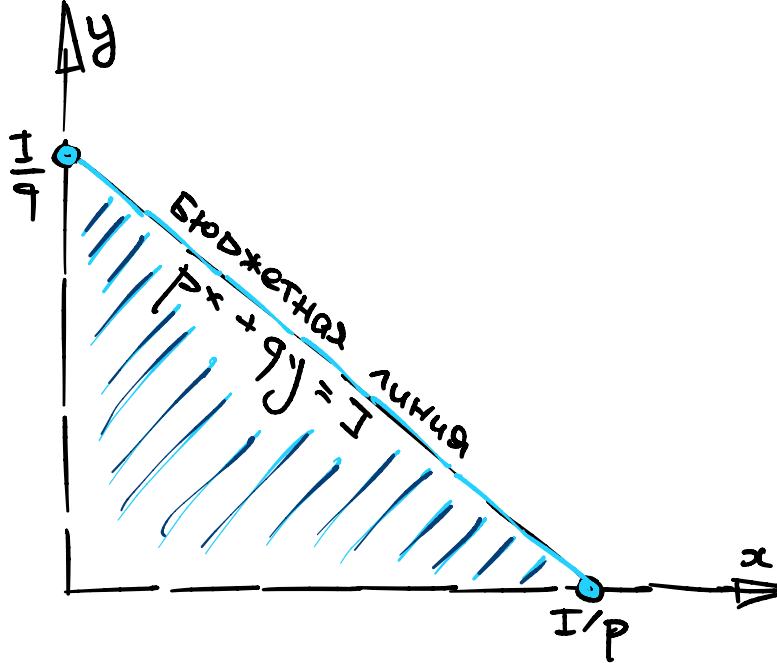
\includegraphics[width=.8 \textwidth]{budget_2d.png}
\end{figure}

\end{frame}

\section{Метод Лагранжа}

\begin{frame}{Метод Лагранжа}

Запишем нашу оптимизационную задачу в следующем виде:
$$ U(x, y) \to \max_{(x,y) \in \mathbb{R}^2_{+}} \quad s.t.\quad  B(x,y) \leqslant 0$$

Тогда Лагранжиан принимает вид:
$$ \mathcal{L}(x, y | \lambda) = U(x,y) - \lambda B(x,y)$$

Знак перед множителем Лагранжа важен в доказательствах, но на практике  не играет роли и можно ставить любой.

Традиция такова, что $\lambda I$ должен войти с плюсом.

\end{frame}

\begin{frame}{Метод Лагранжа}

Далее алгоритм предписывает найти безусловный экстремум Лагранжиана в пространстве $(x, y, \lambda)$, игнорируя ограничения.
$$ \mathcal{L}'_x = 0, \quad \mathcal{L}'_y = 0, \quad \mathcal{L}'_{\lambda} = 0.$$
Это система из трех уравнений с тремя неизвестными.

Таким образом, задача условной оптимизации сводится к безусловной. Однако, не совсем понятно, почему метод Лагранжа вообще работает и что он находит.

\end{frame}

\section{Выпуклая интерпретация ММЛ}

\begin{frame}{Выпуклая интерпретация ММЛ}

Если Лагранжиан (квази) вогнутый по товарам $x,y$ то можно применить, так называемый, \textbf{Сильный Принцип Лагранжа}:
$$ \min_{\lambda \geqslant 0} \max_{x(\lambda),y(\lambda) \geqslant 0} \mathcal{L}(x,y | \lambda) = \textcolor{red}{\max_{x,y \geqslant 0} \min_{\lambda(x,y) \geqslant 0} \mathcal{L}(x,y | \lambda)} $$ 

Справа стоит негладкая задача, эквивалентная условной оптимизации, поскольку $\lambda(x,y)$ выбирается так, чтобы наказать бесконечно отрицательной полезностью в случае выхода за ограничение.

\end{frame}

\begin{frame}{Выпуклая интерпретация ММЛ}

Если Лагранжиан (квази) вогнутый по товарам $x,y$ то можно применить, так называемый, \textbf{Сильный Принцип Лагранжа}:
$$ \textcolor{red}{\min_{\lambda \geqslant 0} \max_{x(\lambda),y(\lambda) \geqslant 0} \mathcal{L}(x,y | \lambda)} =  \max_{x,y \geqslant 0} \min_{\lambda(x,y) \geqslant 0} \mathcal{L}(x,y | \lambda) $$ 

Слева стоит гладкая задача, у которой есть один экстремум типа <<седло>>, а значит его можно найти обыкновенными условиями первого порядка:
$$ \nabla_{(x,y)} \mathcal{L} = 0, \quad \nabla_{\lambda} \mathcal{L} = 0.$$

В выпуклом случае, координаты решения двух задач, а также, значение целевой функции совпадают. Это называется \textbf{Теоремой о Минимаксе}, или \textbf{Сильной Дуальностью}.

\end{frame}

\section{Невыпуклая интерпретация ММЛ}

\begin{frame}{Невыпуклая интерпретация ММЛ}

В общем случае, технология поиска оптимума опирается на, так называемые, \textbf{условия Каруш-Кун-Такера}. Основная идея такова, что градиент целевой функции и градиент активного ограничения должны быть параллельны друг другу:
$$ \nabla_{(x,y)}U - \lambda \nabla_{(x,y)} B = 0$$

Это называется необходимыми условиями первого порядка. Удивительным образом, это совпадает с поиском седла Лагранжиана. Также, там есть условия невязки, о которых я упомяну чуть позже.

\end{frame}

\begin{frame}{Невыпуклая интерпретация ММЛ}

В общем случае, технология поиска оптимума опирается на, так называемые, \textbf{условия Каруш-Кун-Такера}. 

Основная идея такова, что градиент целевой функции и градиент активного ограничения должны быть параллельны друг другу:
$$ \nabla_{(x,y)}U - \lambda \nabla_{(x,y)} B = 0$$

Это называется необходимыми условиями первого порядка, или сокращенно \textbf{УПП} (в англ. \textbf{FOC}). Удивительным образом, это совпадает с поиском седла Лагранжиана.

\end{frame}

\begin{frame}{Невыпуклая интерпретация ММЛ}

Далее надо сделать еще один шаг и проверить достаточные условия второго порядка, или сокращенно \textbf{УВП} (в англ. \textbf{SOC}):
$$ \nabla^2_{(x,y)}U - \lambda \nabla^2_{(x,y)} B \leqslant 0$$

на касательном к ограничении пространстве. Еще более удивительным образом, это совпадает с проверкой (как бы локально) квази вогнутости Лагранжиана в точке.

\end{frame}


\section{Угловые решения}

\begin{frame}{Угловые решения}

На самом деле, поскольку мы оптимизируем в $\mathbb{R}^n_{+}$ в Лагранжиан стоило бы добавить еще дополнительные члены, по одному на каждый товар. 
$$ \mathcal{L}(x,y | \lambda, \ldots) = U(x,y) - \lambda B(x,y) - \ldots$$

Однако, в экономических приложениях, как правило, решение внутреннее. А когда оно не внутреннее, его очень легко отыскать по координатам бюджетного ограничения.

\end{frame}

\section{Значение Лагранжиана в оптимуме}

\begin{frame}{Значение Лагранжиана в оптимуме}

Вспомним условие невязки из курса мат. анализа:

$$ \lambda^{\ast} B(x^{\ast},y^{\ast}) = 0.$$

Оно означает, что одно из двух обязательно верно: либо множитель Лагранжа равен нулю, либо оптимум достигается на границе бюджетного ограничения.

Это значит, что в оптимуме, значение Лагранжиана совпадает со значением целевой функцией:
$$ \mathcal{L}(x^{\ast}, y^{\ast} | \lambda^{\ast}) = U(x^{\ast}, y^{\ast}) - \lambda B(x^{\ast}, y^{\ast})$$ 

Это нам пригодится, когда мы будем изучать ее.

\end{frame}

\section{Интерпретация $\lambda$}

\begin{frame}{Интерпретация $\lambda$}

У множителя $\lambda$ в Лагранжиане есть особая интерпретация, это теневая цена нарушения ограничения:
$$\mathcal{L} = U(x,y) - \lambda B(x,y), \quad B(x,y) \leqslant 0$$ 

Если вам очень хочется выйти за ограничение, Лагранж разрешает вам это сделать, то придется дать (кому-то абстрактно) взятку размера $\lambda$. Рынок подстроится таким образом, что вы не захотите эту взятку давать. 

\end{frame}

\section{Функции спроса}

\begin{frame}{Функции спроса}

Нас будут интересовать координаты оптимума $x^{\ast}(p,q,I)$, $y^{\ast}(p,q,I)$ в задаче максимизации полезности, при бюджетном ограничении, как функции от цен $p,q$ и бюджета $I$. 

\begin{definition}
- кривые "цена-потребление" $x^{\ast}(p, \ldots)$, $y^{\ast}(q, \ldots)$, обычно называемые просто **кривые спроса**.
\end{definition}

\begin{definition}
- кривые "доход-потребление" $x^{\ast}(I, \ldots)$, $y^{\ast}(I, \ldots)$, также называемые **кривые Энгеля** в честь немецкого статистика Эрнста Энгеля (Engel).
\end{definition}

Они также называются \textbf{функциями (кривыми) спроса}.

\end{frame}

\section{Конец}



\end{document}